\chapter{Free Body Diagrams}

Now that you've mastered modeling \textit{how things move}, you can learn to 
model \textit{why things move}. Recall Newton's Second Law:
$$F = ma$$

This is a simplification: what Newton's Second Law says in total is "the 
acceleration of a body is directly proportional to the \textit{net force} 
acting on the body and inversely proportional to the mass of the body." 
Mathematically, that would be:
$$a = \frac{\Sigma F}{m}$$

Where $\Sigma F$ is the vector sum of all the individual forces acting on the 
body. This sum is also called the \textit{net force}. To visualize the magnitude 
and direction of the net force, it can be very helpful to draw a free body 
diagram. 

\section{Interpreting Free Body Diagrams}
Before you learn to draw your own free body diagrams (FBDs), let's examine and 
analyze a few. Here is a FBD for an accelerating car:

\begin{center}
    \begin{tikzpicture}
        \draw[thick] (-1, -1) rectangle (1, 1);
        \draw[fill=black] (0,0) circle (0.4mm);
        \draw[-latex] (0, 0) -- (0, -3) node[below] {$F_g$};
        \draw[-latex] (0,0) -- (-1.25, 0) node[left] {$F_f$};
        \draw[-latex] (0,0) -- (0, 3) node[above] {$F_N$};
        \draw[-latex] (0,0) -- (2, 0) node[right] {$F_{engine}$};
        
    \end{tikzpicture}
\end{center}

We can consider the $x$ and $y$ axes separately. On the $y$-axis, we see that 
the weight ($F_g$) is the same magnitude as the normal force ($F_N$) because the arrows are the same length. This 
means in the $y$ direction, the forces are balanced, and thus we do not expect 
to see acceleration in the $y$ direction. This makes intuitive sense: if you are 
accelerating your car on a flat road, your car does not go up into the air. How 
about the $x$ direction? Here we see friction ($F_f$) pulling the car backwards 
while the engine is pushing the car forwards. In this case, the forces are 
\textit{not} balanced. See how the $F_{engine}$ arrow is longer than the $F_f$ 
arrow? This means the forward force from the engine is \textit{greater in magnitude}
than the backward force of $F_f$. Therefore, the \textit{net force} in the $x$ 
direction is to the right, and the car will accelerate to the right. 

%Here's a more complicated example, where not all the forces are perpendicular to 
%each other. Consider a child sledding down a hill:
%\begin{center}
%\includegraphics[width=5in]{sledder.png}
%\end{center}

\section{Drawing Free Body Diagrams}

A free body diagram consists of the object, usually represented as a simple 
square, with various arrows representing the forces acting on the object. The 
direction and relative lengths of the arrows show the direction and relative 
strength of the forces. Here is a free body diagram for a 2-kg hammer in free fall 
through the air on Earth:

\begin{center}
    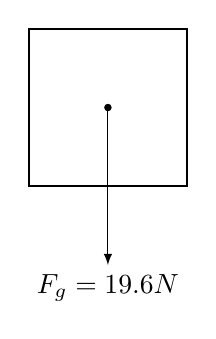
\begin{tikzpicture}
        \draw[thick] (-1, -1) rectangle (1, 1);
        \draw[fill=black] (0,0) circle (0.4mm);
        \draw[-latex] (0, 0) -- (0, -2) node[below] {$F_g = 19.6N$};
    \end{tikzpicture}
\end{center}

% Both methods are useful; choose the one that you prefer. 

\subsection{Objects At Rest}
If an object is at rest, then its acceleration must be $0 \frac{m}{s^2}$. By 
Newton's Second Law, the \textit{net force} acting on that object must also be 
zero. Does this mean there are no forces acting on the object? NO! It means all 
the forces are \textit{balanced}: for every upwards force, there is an equal 
downwards force, and so on. Consider the same 2-kg hammer, but this time it is 
sitting on a table. We know gravity must be acting on the hammer, so let's begin 
with that:

\begin{center}
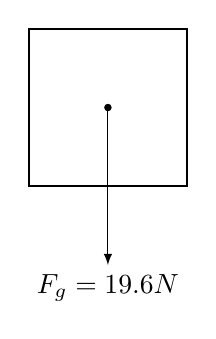
\begin{tikzpicture}
 	\draw[thick] (-1, -1) rectangle (1, 1);
    \draw[fill=black] (0,0) circle (0.4mm);
    \draw[-latex] (0, 0) -- (0, -2) node[below] {$F_g = 19.6N$};
\end{tikzpicture}
\end{center}
% FIXME 
\begin{Exercise}[title = {Blocks on a Table}, label = block1]
[This exercise was originally presented as a free-response question on the 2015 
AP Physics 1 exam.] Two blocks are connected with a string and two pulleys over 
a table, as shown in the figure. Block 1 has a mass of 3 kg and Block 2 has a 
mass of 9 kg. The blocks are released from rest. Treat the string as massless 
and the pulleys as massless and frictionless when answering the questions below. 

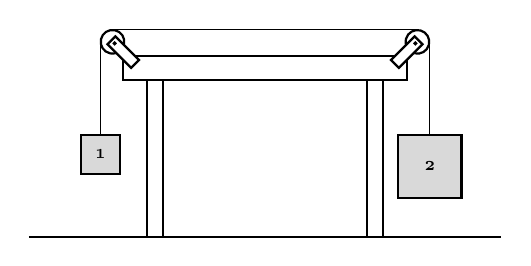
\begin{tikzpicture}
        \draw[thick] (-3, 0) -- (3, 0);
        \draw[thick] (-1.5, 0) rectangle (-1.3, 2);
        \draw[thick] (1.5, 0) rectangle (1.3, 2);
        \draw[thick] (-1.8, 2) rectangle (1.8, 2.3);
        \draw[draw = black, thick, fill=white] (-1.7, 2.15) -- (-1.6, 2.25) -- (-1.9, 2.55) -- (-2, 2.45) -- cycle; 
        \draw[draw=black, thick, fill=white] (1.7, 2.15) -- (1.6, 2.25) -- (1.9, 2.55) -- (2, 2.45) -- cycle;
        \draw[thick, fill=black] (-1.91, 2.46) circle (0.1mm);
        \draw[thick] (-1.79, 2.45) arc (-12:285:0.15);
        \draw[thick, fill=black] (1.91, 2.46) circle (0.1mm);
        \draw[thick] (1.897, 2.335) arc (-105:192:0.15);
        \draw[thin] (-1.94, 2.6382) -- (1.94, 2.6382);
        \draw[thin] (-2.0935, 2.49) -- (-2.0935, 1.3);
        \draw[thin] (2.0927, 2.49) -- (2.0927, 1.3);
        \draw[thick, draw = black, fill = gray!30] (-2.34, 1.3) rectangle (-1.84, 0.8);
        \node[font = \tiny] at (-2.09, 1.05) {\textbf{1}};
        \draw[thick, draw = black, fill = gray!30] (1.69, 1.3) rectangle (2.4954, 0.4946);
        \node[font = \tiny] at (2.0927, 0.8973) {\textbf{2}};
    \end{tikzpicture}
    
\begin{enumerate}
\item Draw free body diagrams for both blocks. Correctly show the relative 
magnitude of the forces using the relative lengths of the vectors. 
\item Before doing any calculations, describe each block's acceleration as (a) 
positive or negative, (b) having a magnitude greater or less than \textit{g}. 
Take the upward direction as positive. 
\item Calculate the acceleration of each block. Take the upward direction as 
positive and express your answer in terms of \textit{g}. 
\end{enumerate}
\end{Exercise}

\begin{Answer}[ref = block1]
\begin{enumerate}
    \item Each block is acted on by gravity and the tension of the string. The 
    force of gravity on block 2 is 3 times that of block 1, and the tension 
    vector should be between the lengths of the gravity vectors:
    \begin{center}
        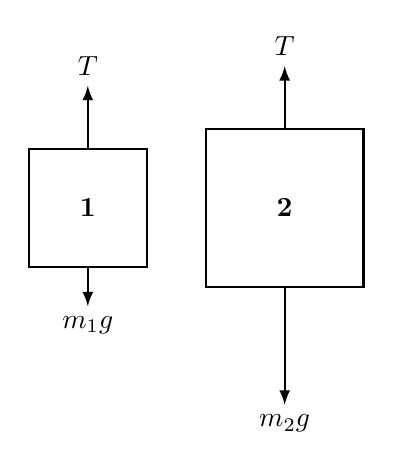
\begin{tikzpicture}
            \draw[thick] (-2, 1) rectangle (-0.5, -0.5);
            \draw[thick] (2.25, 1.25) rectangle (0.25, -0.75);
            \node[] at (-1.25, 0.25) {\textbf{1}};
            \node[] at (1.25, 0.25) {\textbf{2}};
            \draw[thick, -latex] (-1.25, -0.5) -- (-1.25, -1) node[below] {$m_1g$};
            \draw[thick, -latex] (-1.25, 1) -- (-1.25, 1.8) node[above] {$T$};
            \draw[thick, -latex] (1.25, -0.75) -- (1.25, -2.25) node[below] {$m_2g$};
            \draw[thick, -latex] (1.25, 1.25) -- (1.25, 2.05) node[above] {$T$};
        \end{tikzpicture}
    \end{center}

    \item Block 1 will have a positive acceleration with a magnitude less than 
    \textit{g}. Block 2 will have a negative acceleration with a magnitude 
    greater than \textit{g}.

    \item Since the blocks are connected, they will move as a system and 
    therefore have the same magnitude acceleration. From this, the free body 
    diagrams, and Newton's Second Law, we know that:
    $$m_1 a  = T - m_1 g$$
    $$m_2 \left( - a \right) = T - m_2 g$$

    We know $m_1$ and $m_2$, so the two unknowns are $T$ and $a$. One way to 
    solve this system of equations would be to subtract equation 2 from equation 1:
    $$m_1 a + m_2 a = m_2 g - m_1 g$$
    $$a = \frac{m_2 - m_1}{m_1 + m_2} g$$

    Substituting for the masses, we see that:
    $$a = \frac{9 - 3}{9 + 3}g = \frac{6}{12}g = \frac{1}{2}g$$

    Therefore, Block 1 is accelerating at $+\frac{1}{2}g$ and Block 2 is 
    accelerating at $-\frac{1}{2}g$.
\end{enumerate}
\end{Answer}

Now here's an interesting question: what happens if we add another mass to the 
system? Imagine that a third block with a mass of 15 kg is laid on the table 
from the previous exercise and the string is attached to each side, as shown 
below. 
\begin{center}
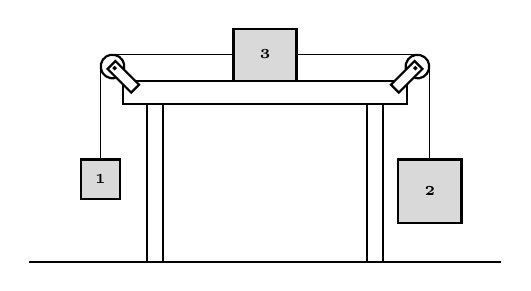
\begin{tikzpicture}
        \draw[thick] (-3, 0) -- (3, 0);
        \draw[thick] (-1.5, 0) rectangle (-1.3, 2);
        \draw[thick] (1.5, 0) rectangle (1.3, 2);
        \draw[thick] (-1.8, 2) rectangle (1.8, 2.3);
        \draw[draw = black, thick, fill=white] (-1.7, 2.15) -- (-1.6, 2.25) -- (-1.9, 2.55) -- (-2, 2.45) -- cycle; 
        \draw[draw=black, thick, fill=white] (1.7, 2.15) -- (1.6, 2.25) -- (1.9, 2.55) -- (2, 2.45) -- cycle;
        \draw[thick, fill=black] (-1.91, 2.46) circle (0.1mm);
        \draw[thick] (-1.79, 2.45) arc (-12:285:0.15);
        \draw[thick, fill=black] (1.91, 2.46) circle (0.1mm);
        \draw[thick] (1.897, 2.335) arc (-105:192:0.15);
        \draw[thin] (-1.94, 2.6382) -- (1.94, 2.6382);
        \draw[thin] (-2.0935, 2.49) -- (-2.0935, 1.3);
        \draw[thin] (2.0927, 2.49) -- (2.0927, 1.3);
        \draw[thick, draw = black, fill = gray!30] (-2.34, 1.3) rectangle (-1.84, 0.8);
        \node[font = \tiny] at (-2.09, 1.05) {\textbf{1}};
        \draw[thick, draw = black, fill = gray!30] (1.69, 1.3) rectangle (2.4954, 0.4946);
        \node[font = \tiny] at (2.0927, 0.8973) {\textbf{2}};
        \draw[thick, draw = black, fill = gray!30] (-0.4, 2.3) rectangle (0.4, 2.96);
        \node[font = \tiny] at (0, 2.638) {\textbf{3}};
    \end{tikzpicture}
\end{center}

We could redraw free body diagrams for all three blocks, noting that the 
tensions on either side of Block 3 will be different. Then, we would have 
another system of equations to solve and we could find the acceleration. Or, 
we could think about the entire system. Originally, the net force on the 
two-block system was 58.8 Newtons (the weight of the larger block minus the 
weight of the smaller block). And the mass of the entire two-block system was 
12 kilograms. We can apply Newton's Second Law:
$$a = \frac{58.8 N}{12 kg} = 4.9 \frac{m}{s^2} = \frac{1}{2}g$$

(Notice, this is the same answer we found in the previous exercise). What 
changes when we add a third, 15-kg block? The net force on the system doesn't 
change: the table pushes back up on the third block with a force equal to the 
block's weight. However, the total mass of the system has changed: it's 
increased. Now the total mass is 27 kg, and we can again apply Newton's Second 
Law:
$$a = \frac{58.8 N}{27 kg} \approx 2.18 \frac{m}{s^2}$$

This answer makes sense: the mass of the system has increased while the net 
force acting on the system has stayed the same, resulting in a slower acceleration. 

Now, what if instead of blocks resting on level tables, the blocks were on an incline? Let's take a look at this and more FBD's in the next chapter.